\documentclass{sig-alternate-ipsn13}

\usepackage{graphicx}
\usepackage{amsmath}
\usepackage[caption=false,font=footnotesize]{subfig}

\DeclareMathOperator{\median}{median}
\DeclareMathOperator{\dis}{d}
\DeclareMathOperator{\mad}{MAD}

\title{Energy Headhunter: \\An Energy-Savings Search Tool for Buildings}
% Mining Devices Intrinsic-Relationships to Identify Energy Saving Opportunities in Buildings


% \numberofauthors{8}
% \author{
% \alignauthor Romain Fontugne
% \alignauthor Jorge Ortiz
% \alignauthor Kensuke Fukuda 
% \alignauthor Nicolas Tremblay
% \and
% \alignauthor Pierre Borgnat
% \alignauthor Patrick Flandrin
% \alignauthor David Culler 
% \alignauthor Hiroshi Esaki
% }
% \IEEEauthorblockA{\IEEEauthorrefmark{1}The University of Tokyo
% \hfill \IEEEauthorrefmark{2}University California Berkeley
% \hfill \IEEEauthorrefmark{3}National Institute of Informatics \\
% \IEEEauthorrefmark{4}ENS Lyon
% \hfill \IEEEauthorrefmark{5}JFLI}
% }

\begin{document}
\maketitle

\section{Introduction}
Buildings are one of the prime targets to reduce energy consumption around the world.
In the United States, the second largest energy consumer in the world, buildings account for 41\% of the country's total energy consumption \cite{aer2011}.
The first measure towards reducing the building's energy consumption is to prevent electricity waste, due to the improper use of the buildings equipment.

Large building infrastructure is usually monitored by numerous sensors.
Some of these sensors enable building administrators to view device power-draw in real time.  This allows administrators
 to determine proper device behavior and system-wide inefficiencies.
%,  and identify devices providing inappropriate services.
% sensors providing a service is weird to think about  -- i like how the next paragraph explains it
Detecting misbehaving devices is crucial, as many are sources of energy waste.  % a light not turning on properly is NOT WASTEFUL, but does affect service quality
However, identifying these saving opportunities is impractical for administrators because large buildings usually contain hundreds of monitored devices
producing thousands of streams and it requires continuous monitoring. % attention as abnormal usages may happen at any time.
%Consequently, the goal of this work is to establish a methodology that reports to building administrators devices abnormal uses.  
As such, the goal of this work is to establish a method that reports abnormal device-usage patterns to the administrator by closely examining 
all of the continuous power streams.

The intuition behind the proposed approach is that each service provided by the building requires a minimum subset of devices.
The devices within a subset are used at the same time when the corresponding service is needed and a savings opportunity is characterized by the partial activation of the devices.
For example, office comfort is attained through sufficient lighting, ventilation, and air conditioning.
These are controlled by the lighting and HVAC system.
%controlled by the lighting system and air conditioner.% the light and air conditioning.
Thus, when the room is occupied both the air conditioner (heater on a cold day) and lights are used together and should be turned off 
when the room is empty.
In principal, if a person leaves the room and turns off \emph{only} the lights then the air conditioner (or heater) is a source of electricity waste.

Following this basic idea we propose an unsupervised methodology to systematically detect electricity waste.
Our proposal consists of two key components:
% \begin{enumerate}
%  \item The strip and bind method (SBM) mines raw sensor data, identifying devices that are used in concert.
%  It uncovers the devices relationships by looking at the correlation of their activities. 
%  Therefore it allows us to differentiate the devices that are used all together (high correlation), devices used independently (no correlation) and the mutually exclusive usages of devices (negative correlation).
%  \item The anomaly detector monitors devices relationships over time and reports misbehaving devices.
%  It learns the devices normal usages using a robust and longitudinal analysis of the building data and detect anomalous usages that stand for electricity wastes.
% \end{enumerate}

\begin{enumerate}
 \item The strip and bind method (SBM) mines the raw sensor data, identifying inter-device usage patterns. % that are typically used in concert to provide a service.
We first \emph{strip} the underlying traces of occupancy-induced trends.  Then we \emph{bind} device traces, whose underlying behavior
is highly correlated, by placing them into a correlated device set.
 %  Then
 % It uncovers the devices relationships by looking at the correlation of their activities. 
 This allows us to differentiate between devices that are used together (high correlation), used independently (no correlation), and used mutually exclusively (negative correlation).
 \item The anomaly detector monitors devices relationships over time and reports deviations from the norm.  % misbehaving devices.
 It learns the normal inter-device usages using a robust, longitudinal analysis of the building data and detect anomalous usage patterns.  Such patterns present an opportunity to reduce electricity waste.
 % that may represent that stand for electricity wastes.
\end{enumerate}

The main challenge we overcame with our approach is uncovering the device relationships from numerous, noisy sensor traces
that all share a similar trend.
%The main difficulty in this approach is to uncover the devices relationship from the numerous and noisy sensor traces. 
Since device energy consumption is mainly driven by building occupancy, all the devices follow the same daily pattern, 
in roughly overlapping time intervals and phases.
%and seem to be used all at once.
Therefore, one of the main contributions of this work is uncovering the intrinsic device relationships by filtering out the dominant
trend.  This is achieved by using Empirical Mode Decomposition \cite{huang:emd1998}.

Another key contribution of this work is in using the SBM method to practically reduce building energy consumption.
Moreover, the proposed method is easy to use and functions in any building, as it does not require prior knowledge of the
 building nor extra sensors.  It is also tuned through a single intuitive parameter.  %which parameter?

We validate the effectiveness of our approach using 10 weeks of data from a modern Japanese building containing 135 sensors and 
8 weeks of data from an older American building containing 70 sensors.
These experiments highlight the effectiveness of SBM to uncover device relationships in a large deployment of 135 sensors.
Furthermore, we inspect the anomaly detector results and show that the reported alarms correspond to significant opportunities to save energy.
The major anomaly reported in the American building accounts for a waste of 2500 kWh over 18 days whereas the building average power consumption is 600 kW per hour.
Without the proposed method identifying these energy wastes would be difficult for building administrators as they are hidden in the building overall consumption.

In the rest of this paper, we detail the mechanisms of SBM and the anomaly detector before evaluating both of them with real data then we discuss different outcomes of the proposed methodology and conclude.


\section{Problem description}
% \subsection{Dominant patterns}
\begin{figure}
\begin{center}
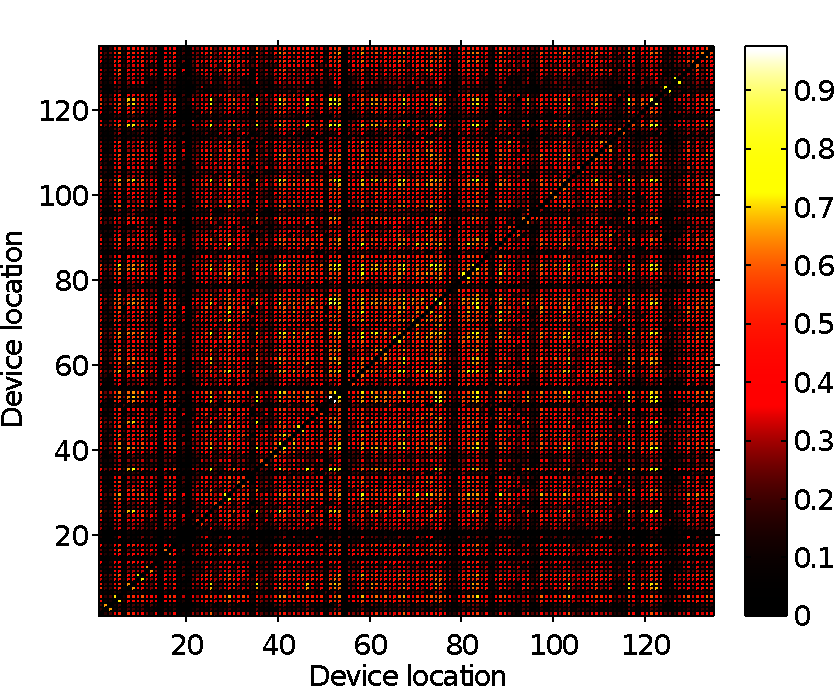
\includegraphics[width=.45\textwidth]{img/heatMap_raw_201106-eps-converted-to.pdf}
\caption{Correlation coefficients of the raw traces from the Engineering Building 2 dataset (Section \ref{data:engbldg2}).
The matrix is ordered such as the devices serving same/adjacent rooms are nearby in the matrix.}
\label{fig:heatmap:raw}
\end{center}
\end{figure}

%The first step of the proposed approach is to uncover from the raw data the devices that are used all together.
The primary objective of SBS is to determine the devices that are used simulataneously.
%The basic tool that allows us to compare device energy consumption is the correlation coefficient.
Initially, we ran correlation analysis across pairs of power-draw signals between distinct devices, summarized by
a correlation coefficient.  However, our results did not yield any useful information when applied to 
the raw data.
%However, during our experiments we found that it provides poor help when it is directly applied to the raw signals.
For example the two raw signals of Figure \ref{fig:diagram1} are from two independent HVAC systems serving different rooms on different floors.
Since each space is independently controlled, we expect their power-draw signals to be uncorrelated (or at least distinguishable 
from other signal pairs).  However, their correlation coefficient ($0.5675$) was not particularly informative.  
% however, their correlation coefficient (i.e. $0.5675$) indicates the opposite.
%Another example, with 135 devices, is depicted in Figure \ref{fig:heatmap:raw}.

% Another example, depicted in Figure \ref{fig:heatmap:raw}, shows a correlation matrix with 135 distinct locations, each containing a number of devices.  
Another example, depicted in Figure \ref{fig:heatmap:raw}, shows a correlation matrix with 135 distinct lighting and HVAC systems serving numerous rooms in a building (Section \ref{data:engbldg2}).
The indices are selected such that their index-difference is indicative of their relative spatial proximity.  
For example, a device in location 1 is closer to a device in location 2 than it is to 
a device in location 135. 
% We do not account for obstructions between them, such as walls.  %?
The color of the cell is the average pairwise correlation coefficient for devices in the row-column index.  The higher the value, the lighter the color.
%the devices serving the same (or adjacent) room are close
%to one another in the matrix.  
Devices serving the same room are along the diagonal.  Because these devices are used simultaneously, we expect
high average correlation scores, lighter shades, along the diagonal figure.
%and because they are used simultaneously by the room users we expect them to feature the highest correlation scores.
However, we observe no such pattern.  %structure is unseen in the Figure.  
Most of the signals are correlated with all the others and we see no discernable structure.
% thus this metric prevents us from finding devices that are used in concert.

\begin{figure}[t!]
\begin{center}
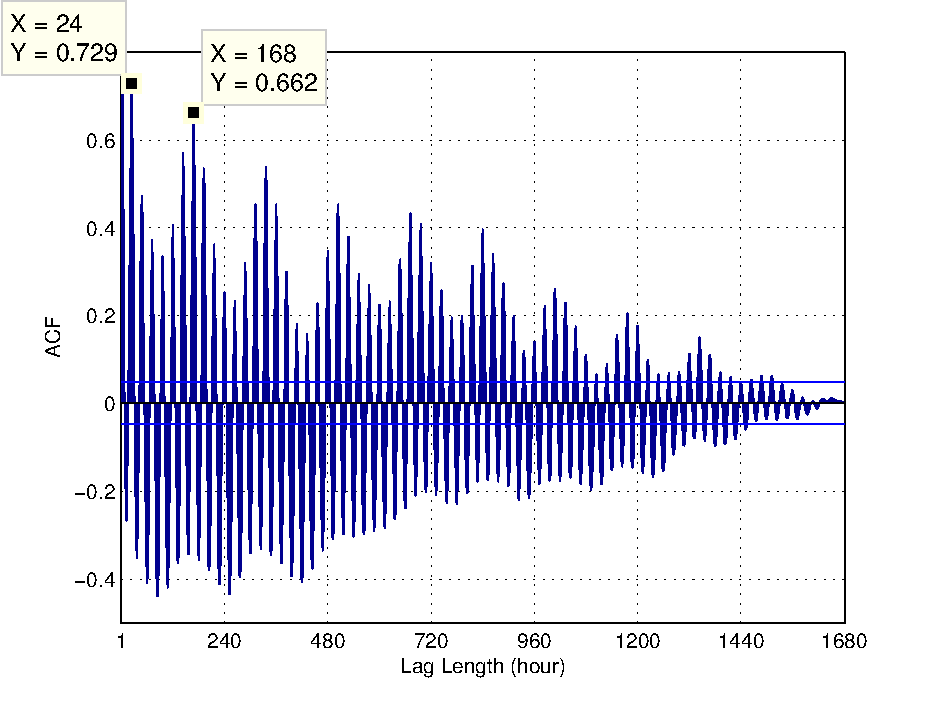
\includegraphics[width=.45\textwidth]{img/acf_101A1_GHP-eps-converted-to.pdf}
\caption{Auto-correlation of a usual signal from the Engineering Building 2 dataset.
The signal features daily and weekly patterns (resp. $x=24$ and $x=168$).}
\label{fig:autocorr}
\end{center}
\end{figure}

Intuitively, the daily occupant usage patterns %office hours, 
drives these results.
Figure \ref{fig:diagram1} demonstrates this more clearly.  It shows two 1-week raw signals traces which feature the same 
diurnal pattern.  
This trend is present in almost every sensor trace, and it hides 
the smaller fluctuations providing more specific patterns driven by local occupant activity.  Upon deeper inspection, we uncovered several
 dominant patterns, common among energy-consuming devices in buildings~\cite{wrinch:pes2012}.  Figure~\ref{fig:autocorr} depicts the 
 auto-correlation of a usual electric power signal for a device.  The two highest values in the figure correspond to a lag of 24 hours and 168 hours (one week).  
 Therefore, the signal is periodic and similar values are seen at daily and weekly time scales.
The daily pattern is due to daily office hours and the weekly pattern corresponds to weekdays and weekends.  
%Indeed, thorough inspection of the data reveals that the 
Clearly, the use of correlation analysis on the \emph{raw} signals reveals no useful information and cannot be used to determine meaningful 
inter-device relationships.  %metric is insufficient with raw signals containing the same dominant pattern.

Such trends must be removed in order to make meaningful progress towards our aforementioned goals.  In the next section
we describe SBS.  We discuss \emph{strip and bind} in section~\ref{methodo:est}, which addresses the detrending and
relationship-discovery challenge.  Then we describe how we \emph{search} for changes in those usage patterns, 
in section~\ref{methodo:ano}, to identify potential opportunities for savings.

%One of the major challenges in this work is to discard these patterns and uncover devices intrinsic relationships.
% This difficulty is overcome by the first part of the method (Strip and Bind) presented in Section \ref{methodo:est}.
% Then, the second part of the method (Search) monitors over time the devices relationships and detect abnormal device behavior changes (Section \ref{methodo:ano}).



\section{Demo description}
We have integrated SBS into a fully functional anomaly detectiong system for building managers.  The system 
is desgined as a web application that take a bulk-data feed, runs SBS on the data, and displays the associated 
signals where anomalies have been detected.  This system address two challenges that are not addressed in the 
paper~\cite{SBS}.  It accepts user input on the anomalies that were detected, so that the system can learn
how to distinguish between a potential false-positive and true-positive.  Secondly, it provides a common vocabulary
to users to help normalize the data across data set and buildings.  A \emph{major} challenge in buildings 
is that the vocabulary and inter-relationships between the sensor, spaces, and sub-system varies slightly
from building to building.  By providing a tagging mechanism, we attempt to embedded symantic information
that, in time, can be used to characterize the classes of anomalies and faults found with the SBS tool.




\small
\bibliographystyle{abbrv}
\bibliography{references}
\end{document}